\documentclass{beamer}
\usepackage{tikz,amsmath,hyperref,graphicx,stackrel,animate,cancel}
\usetikzlibrary{positioning,shadows,arrows,shapes,calc}
\newcommand{\argmax}{\operatornamewithlimits{argmax}}
\newcommand{\argmin}{\operatornamewithlimits{argmin}}
\mode<presentation>{\usetheme{Frankfurt}}
\AtBeginSection[]
{
  \begin{frame}<beamer>
    \frametitle{Outline}
    \tableofcontents[currentsection,currentsubsection]
  \end{frame}
}
\title{Lecture 2: Sines, Cosines and Complex Exponentials}
\author{Mark Hasegawa-Johnson}
\date{ECE 401: Signal and Image Analysis, Fall 2023}  
\begin{document}

% Title
\begin{frame}
  \maketitle
\end{frame}

% Title
\begin{frame}
  \tableofcontents
\end{frame}

%%%%%%%%%%%%%%%%%%%%%%%%%%%%%%%%%%%%%%%%%%%%
\section[Cosines]{Sines and Cosines}
\setcounter{subsection}{1}

\begin{frame}
  \frametitle{SOHCAHTOA}

  Sine and Cosine functions were invented to describe the sides of a right triangle:
  \begin{align*}
    \sin\theta &= \frac{\mbox{Opposite}}{\mbox{Hypotenuse}}\\
    \cos\theta &= \frac{\mbox{Adjacent}}{\mbox{Hypotenuse}}\\
    \tan\theta &= \frac{\mbox{Opposite}}{\mbox{Adjacent}}
  \end{align*}
\end{frame}

\begin{frame}
  \frametitle{SOHCAHTOA}

  \centerline{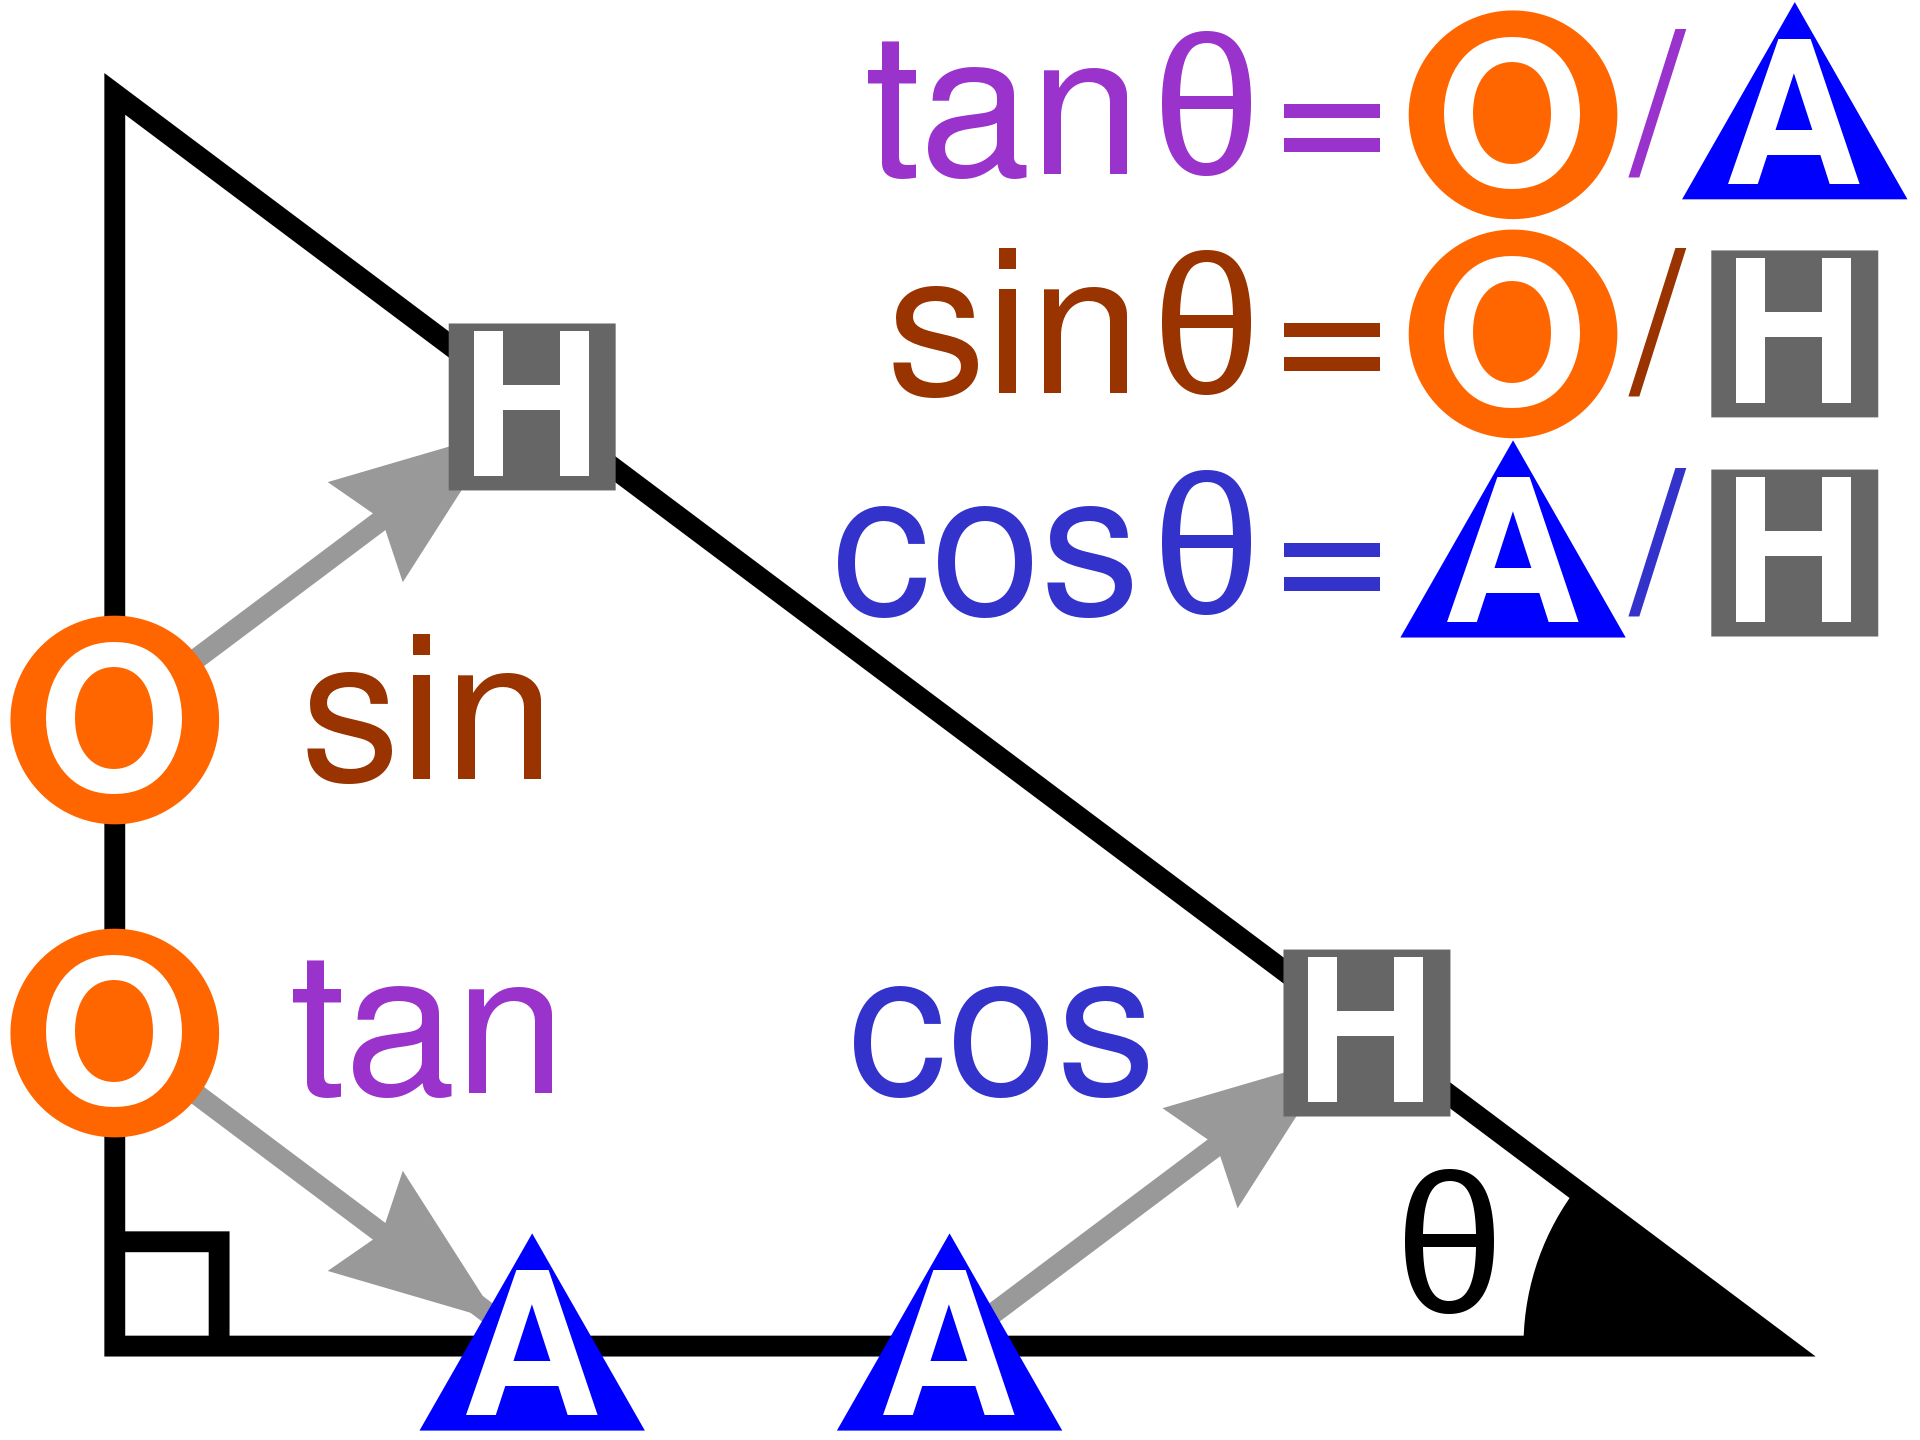
\includegraphics[height=2.5in]{exp/sohcahtoa.png}}
  \begin{tiny}
    By Cmglee, CC-SA 4.0,
    \url{https://commons.wikimedia.org/wiki/File:Trigonometric_function_triangle_mnemonic.svg}
  \end{tiny}
\end{frame}

\begin{frame}
  \frametitle{Sines, Cosines, and Circles}

  Imagine an ant walking counter-clockwise around a circle of radius $A$.
  Suppose the ant walks all the way around the circle once every $T$ seconds.
  \begin{itemize}
  \item The ant's horizontal position at time $t$, $x(t)$, is given by
    \[
    x(t) = A\cos\left(\frac{2\pi t}{T}\right)
    \]
  \item The ant's vertical position, $y(t)$, is given by
    \[
    y(t) = A\sin\left(\frac{2\pi t}{T}\right)
    \]
  \end{itemize}
\end{frame}

\begin{frame}
  \frametitle{Sines, Cosines, and Circles\\\begin{tiny}by Gonfer, CC-SA 3.0,
    \url{https://commons.wikimedia.org/wiki/File:Unfasor.gif}\end{tiny}}
  \centerline{\animategraphics[loop,controls,height=2.5in]{20}{exp/Unfasor-}{0}{47}}
\end{frame}

\begin{frame}
  \frametitle{$x(t)$ and $y(t)$}

  \centerline{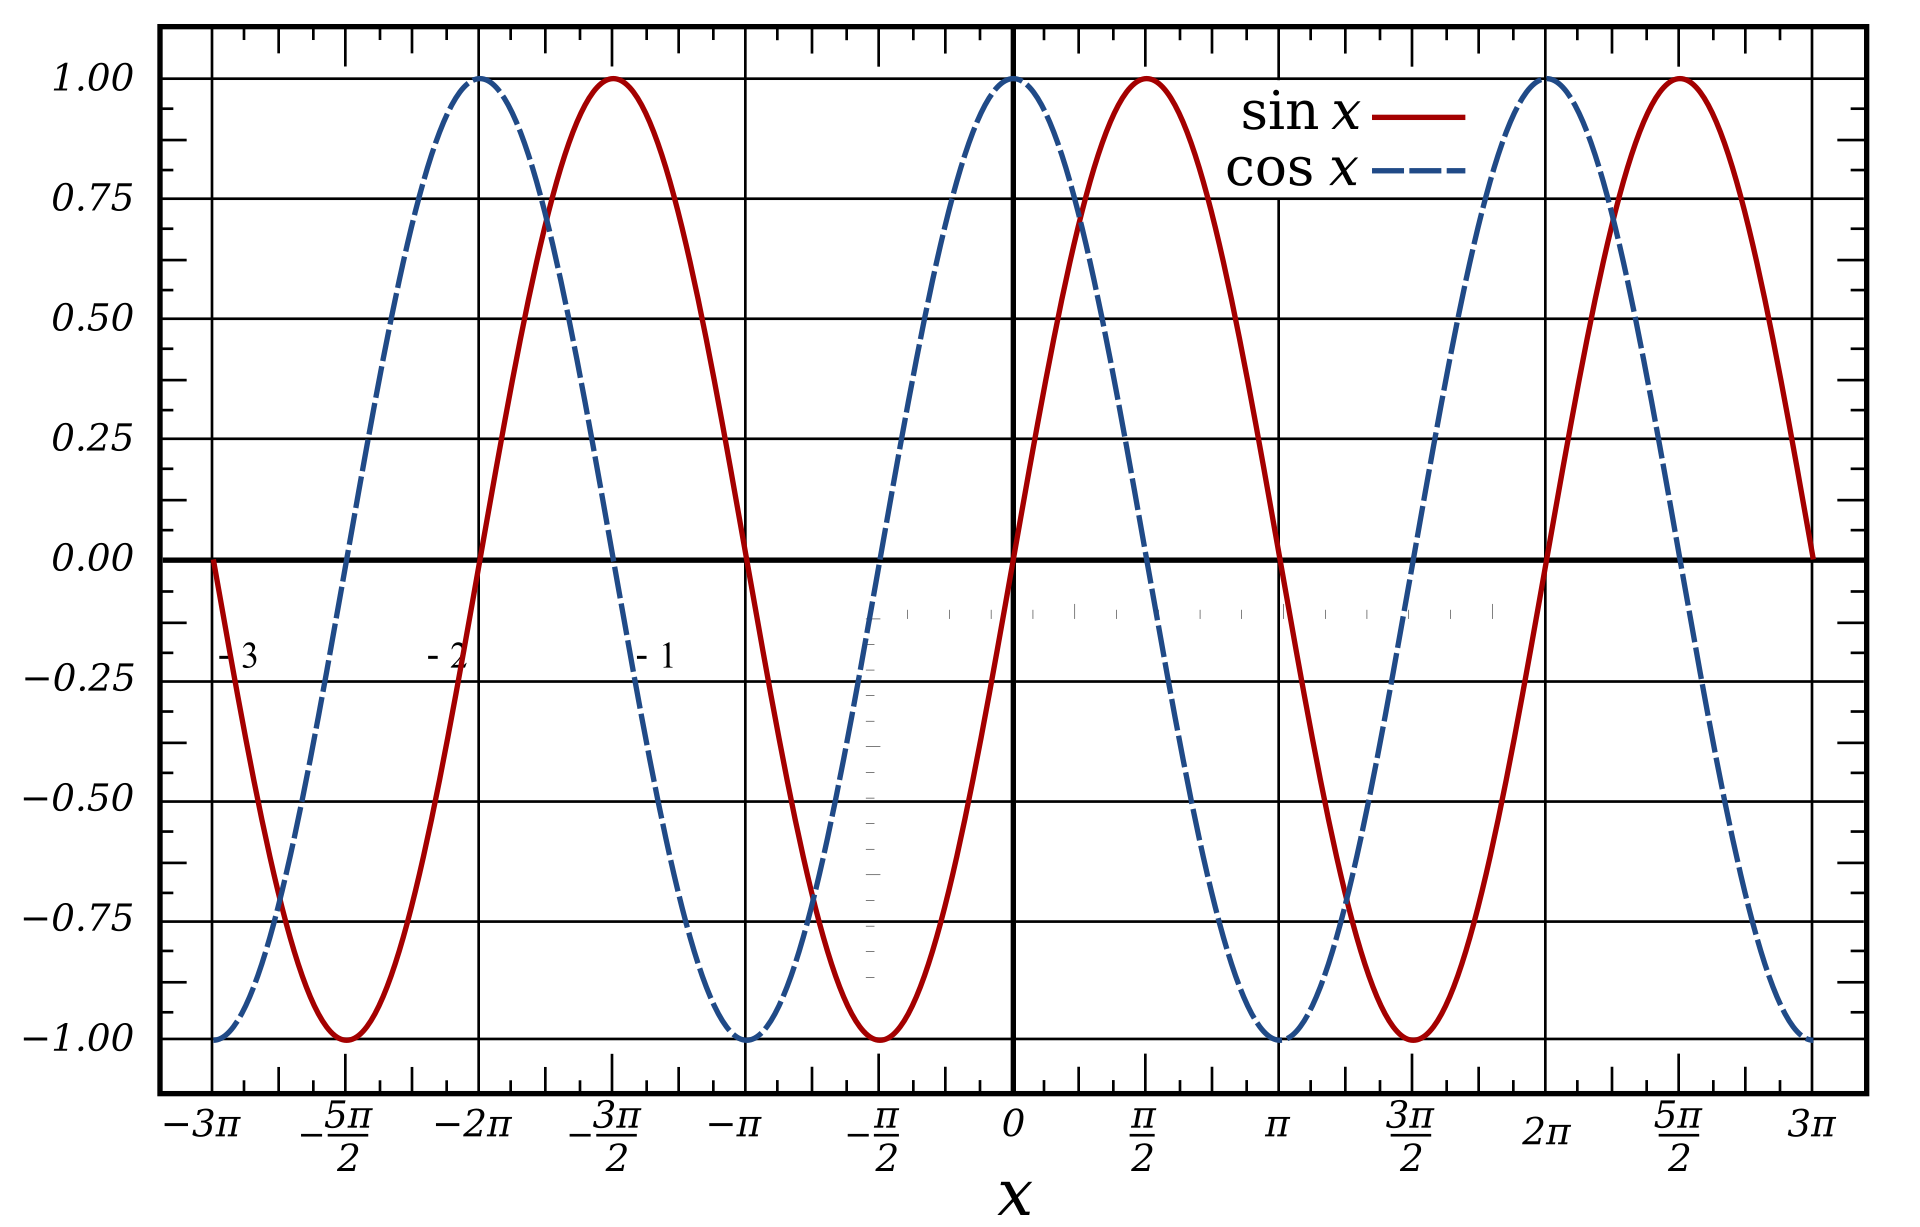
\includegraphics[width=\textwidth]{exp/sine_and_cosine.png}}
  \begin{tiny}
    By Inductiveload, public domain image 2008,
    \url{https://commons.wikimedia.org/wiki/File:Sine_and_Cosine.svg}
  \end{tiny}
\end{frame}

\begin{frame}
  \frametitle{Period and Frequency}

  The period of a cosine, $T$, is the time required for one complete
  cycle.  The frequency, $f=1/T$, is the number of cycles per second.
  This picture shows
  \[
  y(t)  = A\sin\left(\frac{2\pi t}{T}\right) = A\sin\left(2\pi ft\right)
  \]
  \centerline{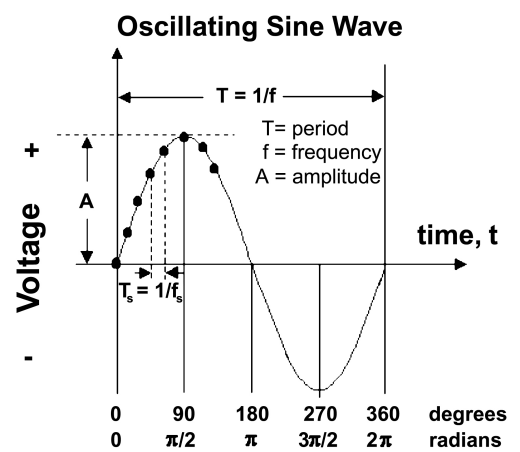
\includegraphics[height=2in]{exp/Oscillating_sine_wave.png}}
\end{frame}  

\begin{frame}
  \frametitle{Pure Tones}
  
  In music or audiometry, a ``pure tone'' at frequency $f$ is an
  acoustic signal, $p(t)$, given by
  \[
  p(t) = A\cos\left(2\pi ft+\theta\right)
  \]
  for any amplitude $A$ and phase $\theta$.
  \vspace*{3mm}
  
  \centerline{\fbox{\href{https://en.wikipedia.org/wiki/Sine_wave}{Pure Tone Demo}}}
\end{frame}
  
\begin{frame}
  \frametitle{Phase, Distance, and Time}
  
  Remember the ant on the circle.  The circle has a radius of $A$ (say, $A$ centimeters).
  \begin{itemize}
  \item When the ant has walked a distance of $A$ centimeters around
    the outside of the circle, then it has moved to an angle of 1 radian.
  \item When the ant walks all the way around the circle, it has
    walked $2\pi A$ centimeters, which is $2\pi$ radians.
  \end{itemize}
\end{frame}

\begin{frame}
  \frametitle{Phase, Distance, and Time}
  \centerline{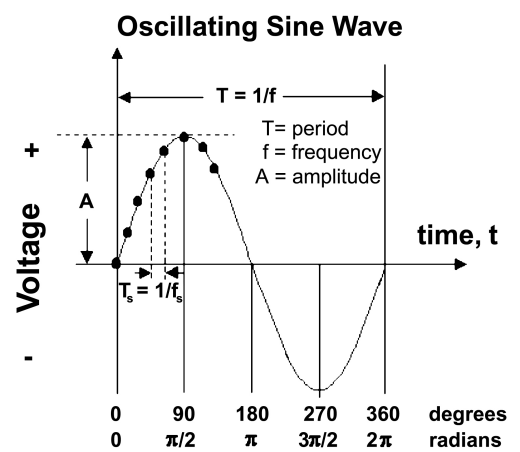
\includegraphics[height=2.5in]{exp/Oscillating_sine_wave.png}}
  \begin{tiny}
    National Institute of Standards and Technology, public domain image 2010
    \url{https://www.nist.gov/pml/time-and-frequency-division/popular-links/time-frequency-z/time-and-frequency-z-p}
  \end{tiny}
\end{frame}

\begin{frame}
  \frametitle{Phase Shift}

  Where did the ant start?
  \begin{itemize}
  \item If the ant starts at an angle of $\theta$, and continues walking counter-clockwise
    at $f$ cycles/second, then
    \[
    x(t) = A\cos\left(\frac{2\pi t}{T}+\theta\right)
    \]
  \item This is exactly the same as if it started walking from phase 0 at time
    $-\tau=-\frac{\theta}{2\pi f}$:
    \[
    x(t) = A\cos\left(\frac{2\pi}{T}\left(t+\tau\right)\right),~~~
    \tau=\frac{T\theta}{2\pi} = \frac{\theta}{2\pi f}
    \]
  \end{itemize}
\end{frame}

\begin{frame}
  \frametitle{Phase Shift}

  Where did the ant start?
  
  \centerline{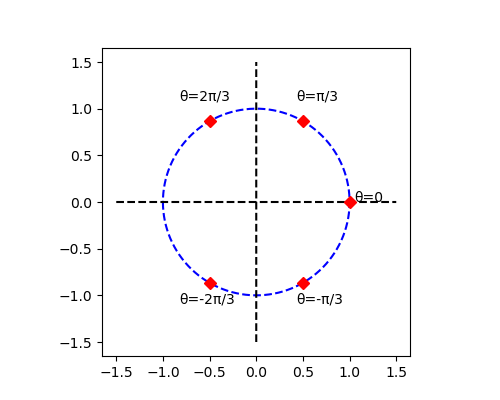
\includegraphics[height=2.5in]{exp/startingpoints.png}}
\end{frame}

\begin{frame}
  \frametitle{Phase Shift}
  
  What is the ant's $x(t)$ position, based on where it started?
  
  \centerline{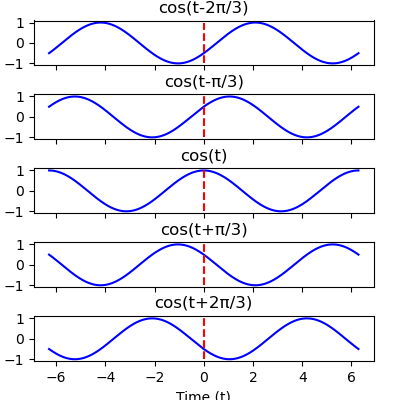
\includegraphics[height=3in]{exp/phaseshift.png}}
\end{frame}

%%%%%%%%%%%%%%%%%%%%%%%%%%%%%%%%%%%%%%%%%%%%
\section[Beating]{Beat Tones}
\setcounter{subsection}{1}

\begin{frame}
  \frametitle{Beat tones}

  When two pure tones at similar frequencies are added together, you hear the  two tones
  ``beating'' against each other.
  \vspace*{1cm}
  \centerline{\fbox{\href{https://en.wikipedia.org/wiki/Beat_(acoustics)}{Beat tones demo}}}
\end{frame}

\begin{frame}
  \frametitle{Beat tones and Trigonometric identities}

  Beat tones can be explained using this trigonometric identity:
  \[
  \cos(a)\cos(b)=\frac{1}{2}\cos(a+b)+\frac{1}{2}\cos(a-b)
  \]
  Let's do the following variable substitution:
  \begin{align*}
    a+b &= 2\pi f_1 t\\
    a-b &= 2\pi f_2 t\\
    a &= 2\pi f_{ave}t\\
    b &= 2\pi f_{beat}t
  \end{align*}
  where $f_{ave}=\frac{f_1+f_2}{2}$, and $f_{beat}=\frac{f_1-f_2}{2}$.
\end{frame}

\begin{frame}
  \frametitle{Beat tones and Trigonometric identities}

  Re-writing the trigonometric identity, we get:
  \[
  \frac{1}{2}\cos(2\pi f_1t)+\frac{1}{2}\cos(2\pi f_2 t) = \cos(2\pi f_{beat}t)\cos(2\pi f_{ave}t)
  \]
  So when we play two tones together, $f_1=110$Hz and $f_2=104$Hz, it
  sounds like we're playing a single tone at $f_{ave}=107$Hz,
  multiplied by a beat frequency $f_{beat}=3$ (double beats)/second.
\end{frame}

\begin{frame}
  \frametitle{Beat tones\\\begin{tiny}by Adjwilley, CC-SA 3.0,
    \url{https://commons.wikimedia.org/wiki/File:WaveInterference.gif}\end{tiny}}
  \centerline{\animategraphics[loop,controls,width=\textwidth]{20}{exp/WaveInterference-}{0}{80}}
\end{frame}


\begin{frame}
  \frametitle{More complex beat tones}

  What happens if we add together, say, three tones?
  \[
  \cos(2\pi 107t) + \cos(2\pi 110t)+\cos(2\pi 104t)=\mbox{???}
  \]
  For this, and other more complicated operations, it
  is much, much easier to work with complex exponentials, instead of cosines.
\end{frame}
  

%%%%%%%%%%%%%%%%%%%%%%%%%%%%%%%%%%%%%%%%%%%%
\section[Phasors]{Phasors}
\setcounter{subsection}{1}

\begin{frame}
  \frametitle{Euler's Identity}

  Euler asked: ``What is $e^{j\theta}$?''  He used the exponential summation:
  \[
  e^{x} = 1 + x + \frac{1}{2}x^2 + \ldots \frac{1}{n!} x^n+\ldots
  \]
  to show that
  \[
  e^{j\theta} = \cos\theta + j\sin\theta
  \]
\end{frame}

\begin{frame}
  \frametitle{Euler's formula}

  \centerline{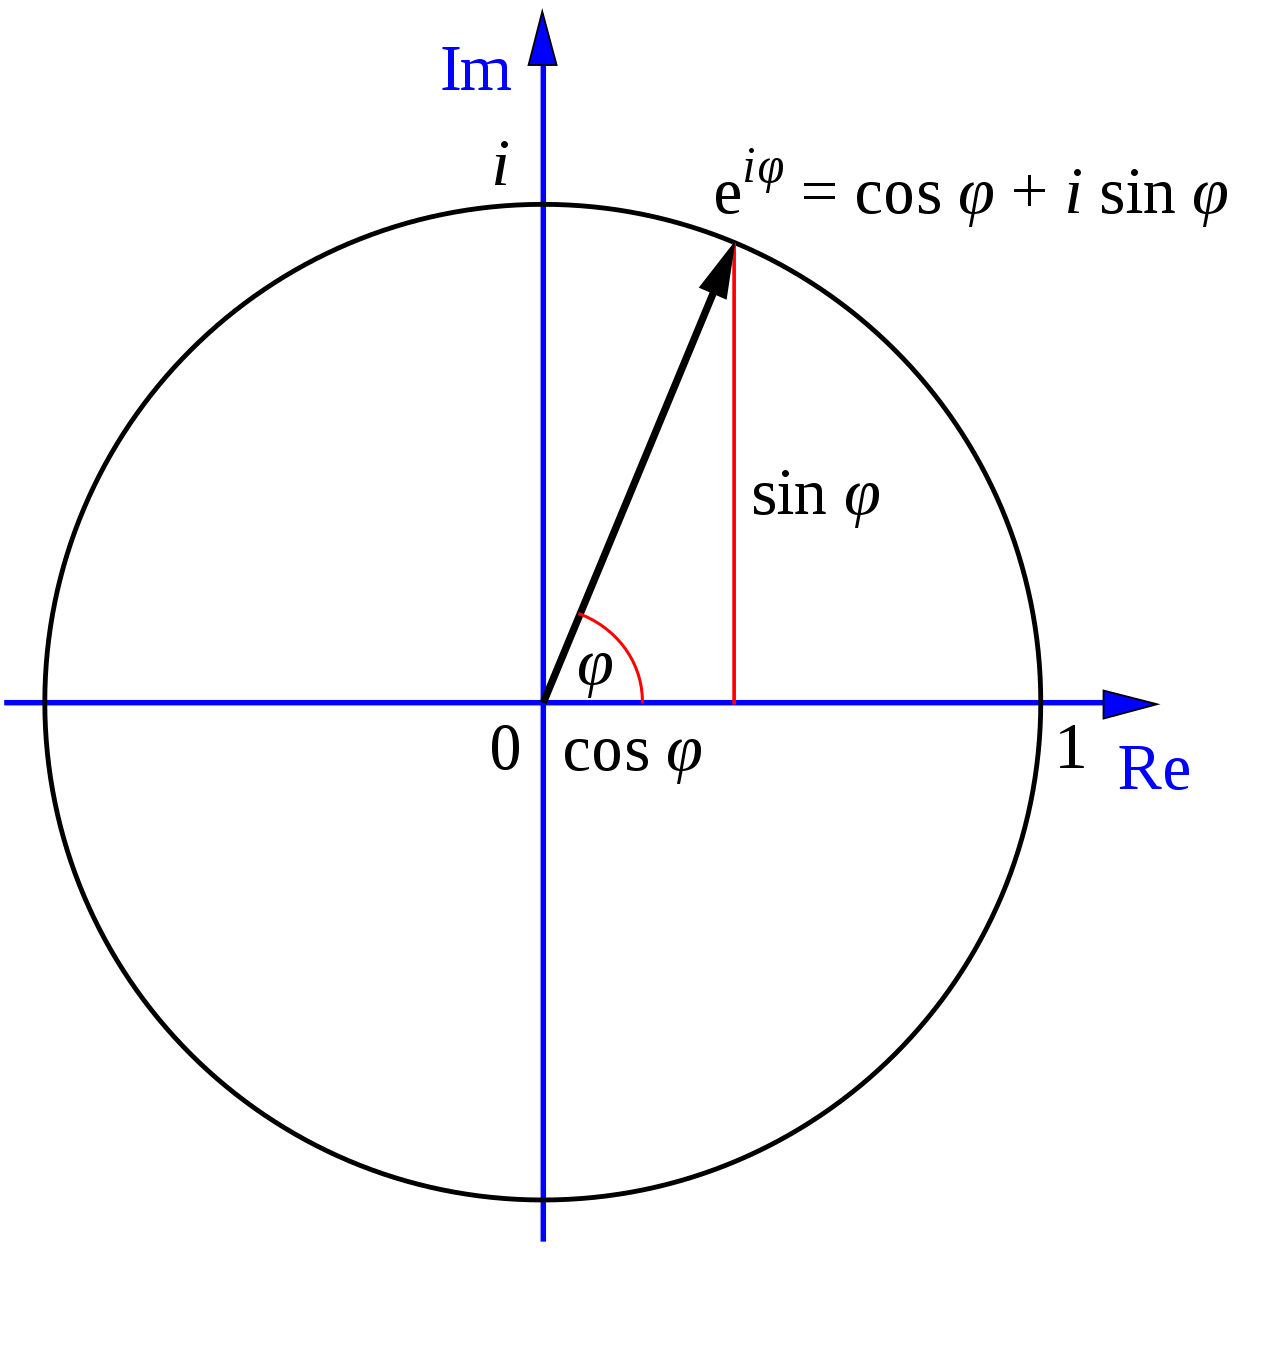
\includegraphics[height=2.5in]{exp/Euler.png}}
  \begin{tiny}
    By Gunther, CC-SA 3.0,
    \url{https://commons.wikimedia.org/wiki/File:Euler\%27s_formula.svg}
  \end{tiny}
\end{frame}

\begin{frame}
  \frametitle{Complex conjugates}

  The polar form of a complex number is $z=re^{j\theta}$,
  \[
  z = re^{j\theta} = r\cos\theta + jr\sin\theta
  \]
  The complex conjugate is defined to be the mirror image of $z$,
  mirrored through the real axis:
  \[
  z^* = re^{-j\theta} = r\cos\theta - jr\sin\theta
  \]
\end{frame}

\begin{frame}
  \frametitle{Complex conjugate}

  \centerline{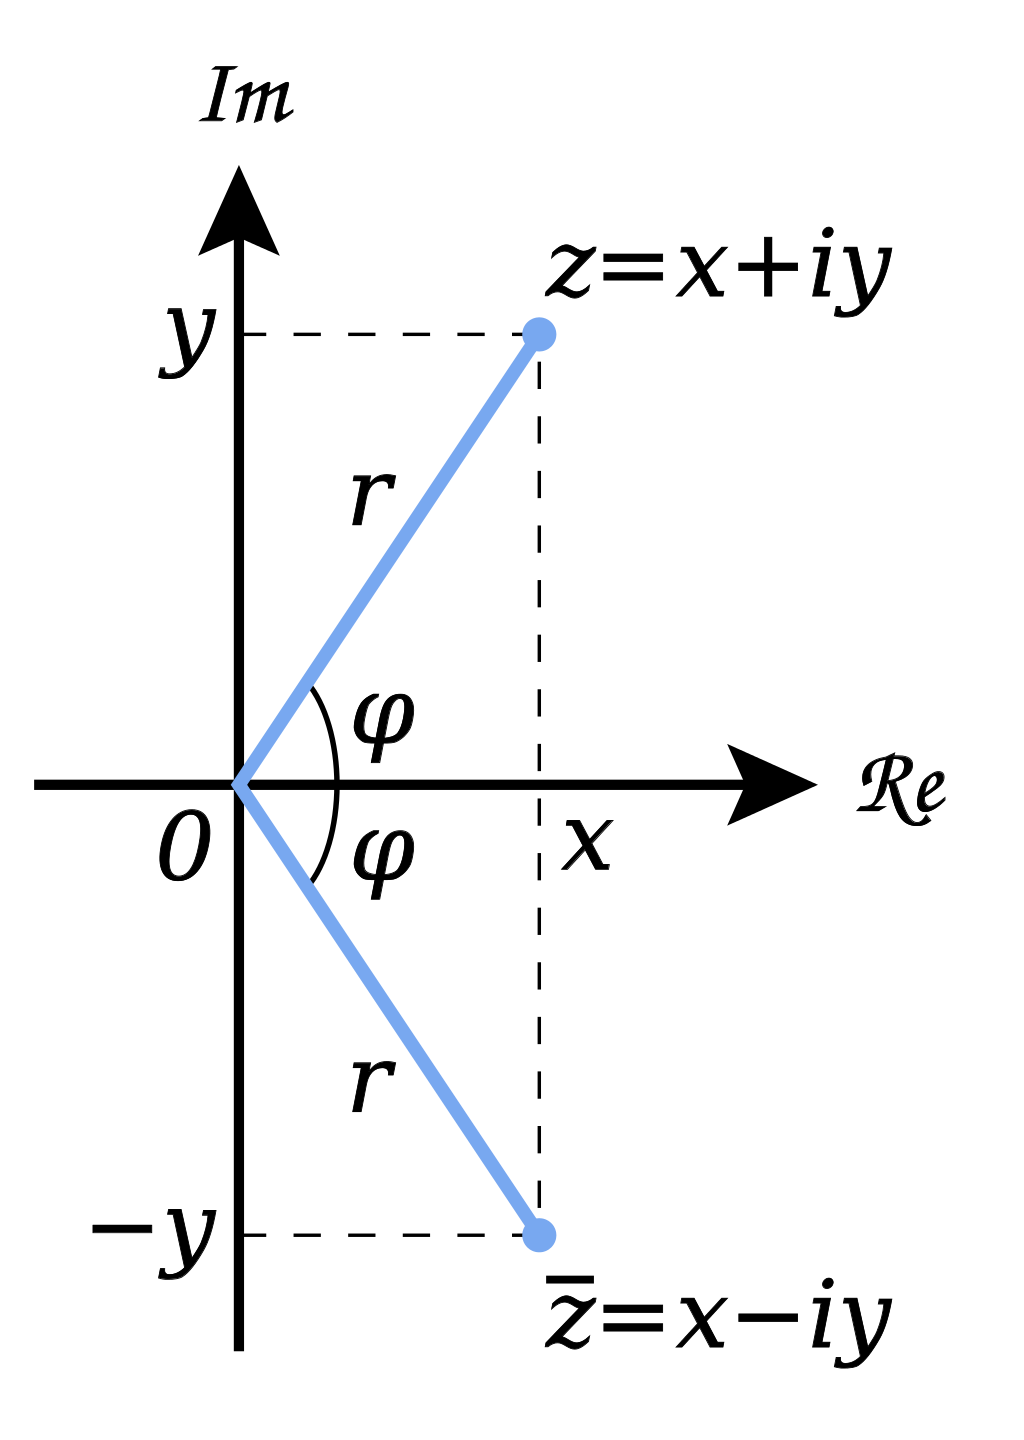
\includegraphics[height=2.5in]{exp/Complex_conjugate_picture.png}}
  \begin{tiny}
    By Oleg Alexandrov, CC-SA 3.0,
    \url{https://commons.wikimedia.org/wiki/File:Complex_conjugate_picture.svg}
  \end{tiny}
\end{frame}

\begin{frame}
  \frametitle{Real part of a complex number}

  If we know $z$ and $z^*$,
  \begin{align*}
  z &= re^{j\theta} = r\cos\theta + jr\sin\theta\\
  z^* &= re^{-j\theta} = r\cos\theta - jr\sin\theta
  \end{align*}
  Then we can get the real part of $z$ back again as
  \[
  \Re\left\{z\right\} = \frac{1}{2}\left(z+z^*\right)
  \]
\end{frame}

\begin{frame}
  \frametitle{Why complex exponentials are better than cosines}

  Suppose we want to add together a lot of phase shifted, scaled
  cosines, all at the same frequency:
  \[
  x(t) = A\cos\left(2\pi ft+\theta\right)+B\cos\left(2\pi ft+\phi\right)+C\cos\left(2\pi ft+\psi\right)
  \]
  What is $x(t)$?
\end{frame}

\begin{frame}
  \frametitle{Why complex exponentials are better than cosines}

  We can simplify this problem by finding the {\bf phasor
    representation} of the tones (I'll give you a formal definition of
  ``phasor'' in a few slides):
  \begin{align*}
    A\cos\left(2\pi ft+\theta\right) &= \Re\left\{Ae^{j\theta}e^{j2\pi ft}\right\}\\
    B\cos\left(2\pi ft+\phi\right) &= \Re\left\{Be^{j\phi}e^{j2\pi ft}\right\}\\
    C\cos\left(2\pi ft+\psi\right) &= \Re\left\{Ce^{j\theta}e^{j2\psi ft}\right\}
  \end{align*}
  So
  \[
  x(t) = \Re\left\{\left(Ae^{j\theta}+Be^{j\phi}+Ce^{j\psi}\right)e^{j2\pi ft}\right\}
  \]
\end{frame}

\begin{frame}
  \frametitle{Why complex exponentials are better than cosines}

  We add complex numbers by (1) adding their real parts, and (2)
  adding their imaginary parts:
  \begin{align*}
    Ae^{j\theta}+Be^{j\phi}+Ce^{j\psi} &= (A\cos\theta+B\cos\phi+C\cos\psi)\\
    &+j(A\sin\theta+B\sin\phi+C\sin\psi)
  \end{align*}
  \centerline{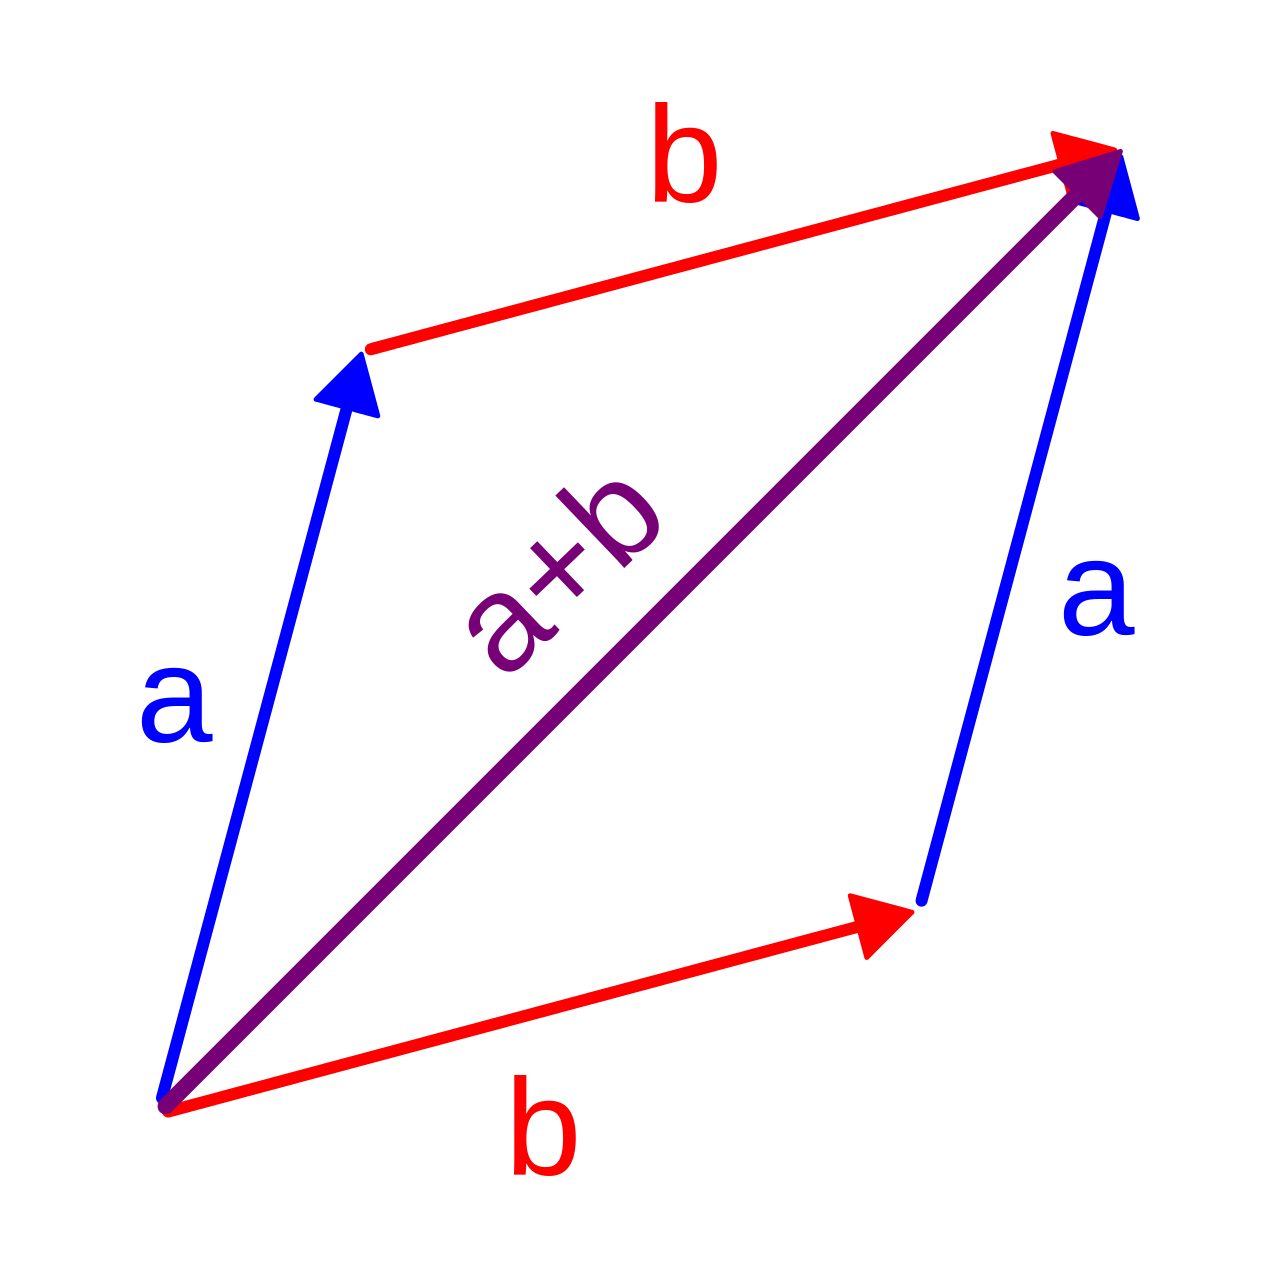
\includegraphics[height=1.75in]{exp/Vector_Addition.png}}
  \begin{tiny}
    By Booyabazooka, public domain image 2009,
    \url{https://commons.wikimedia.org/wiki/File:Vector_Addition.svg}
  \end{tiny}
\end{frame}

\begin{frame}
  \frametitle{Adding phasors\\\begin{tiny} by Gonfer, CC-SA 3.0,
    \url{https://commons.wikimedia.org/wiki/File:Sumafasores.gif}\end{tiny}}
  
  \centerline{\animategraphics[loop,controls,height=2.5in]{20}{exp/Sumafasores-}{0}{47}}
\end{frame}

\begin{frame}
  \frametitle{Why complex exponentials are better than cosines}

  Suppose we want to add together a lot of phase shifted, scaled
  cosines, all at the same frequency:
  \[
  x(t) = A\cos\left(2\pi ft+\theta\right)+B\cos\left(2\pi ft+\phi\right)+C\cos\left(2\pi ft+\psi\right)
  \]
  Here's the fastest way to do that:
  \begin{enumerate}
  \item Convert all the tones to their phasors, $a=Ae^{j\theta}$,
    $b=Be^{j\phi}$, and $c=Ce^{j\psi}$.
  \item Add the phasors: $x=a+b+c$.
  \item Take the real part:
    \[x(t) = \Re\left\{xe^{j2\pi ft}\right\}
    \]
  \end{enumerate}
\end{frame}

\begin{frame}
  \frametitle{BTW, What is a ``phaser''?}
  \centerline{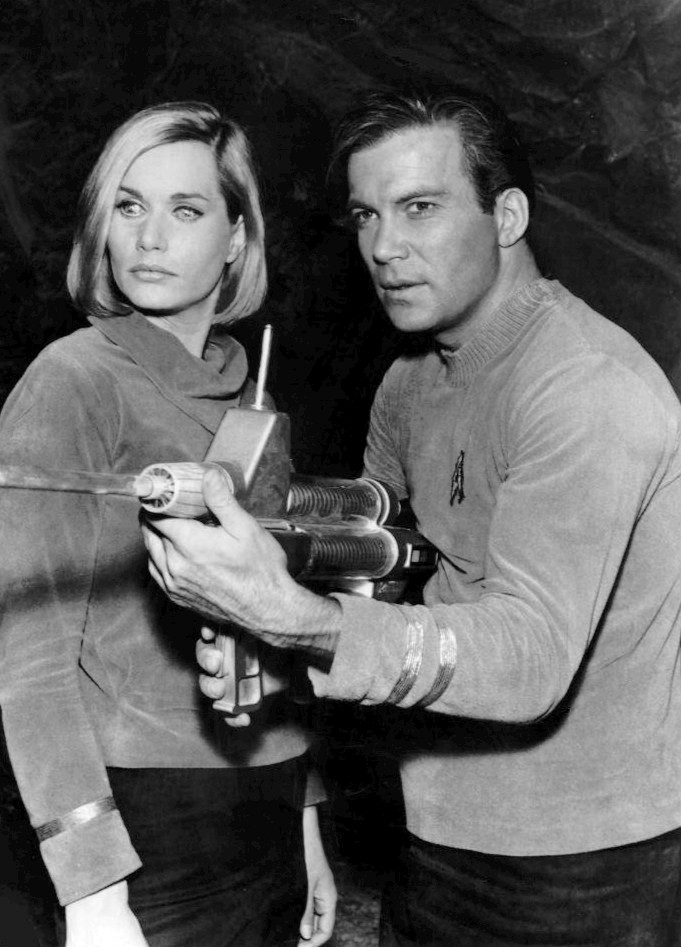
\includegraphics[height=2.5in]{exp/startrek.jpg}}
  \begin{tiny}
    By McFadden, Strauss Eddy \& Irwin for Desilu Productions, public domain image 1966,
    \url{https://commons.wikimedia.org/wiki/File:William_Shatner_Sally_Kellerman_Star_Trek_1966.JPG}
  \end{tiny}
\end{frame}

\begin{frame}
  \frametitle{BTW, What is a \xcancel{``phaser''} ``phasor''?}

  \href{https://en.wikipedia.org/wiki/Phasor}{Wikipedia} has the following definition, which is
  the best I've ever seen:
  \begin{itemize}
    \item The function $Ae^{j(\omega t+\theta)}$ is called the {\bf
      analytic representation} of $A\cos(\omega t+\theta)$.
    \item It is sometimes convenient to refer to the entire function
      as a {\bf phasor}. But the term {\bf phasor} usually implies just the static
      vector $Ae^{j\theta}$.
  \end{itemize}
  In other words, the ``phasor'' can mean either $Ae^{j(\omega
    t+\theta)}$ or just $Ae^{j\theta}$.  If you're asked for the
  phasor representation of some cosine, either answer is correct.
\end{frame}

\begin{frame}
  \frametitle{Some phasor demos from the textbook}

  Here are some phasor demos, provided with the textbook.
  \begin{itemize}
  \item\href{http://dspfirst.gatech.edu/chapters/03spect/demos/phasors/index.html}{\bf\color{blue}One
    rotating phasor demo}: This shows how the cosine, $\cos(2\pi ft
    +\theta)$, is the real part of the phasor $e^{j(2\pi ft+\theta)}$.
  \item\href{http://dspfirst.gatech.edu/chapters/03spect/demos/phasors/index.html}{\bf\color{blue}Positive
    and Negative Frequency Phasors}: This shows how you can get the
    real part of a phasor by adding its complex conjugate (its ``negative frequency phasor''):
    \[
    \cos(2\pi ft+\theta)=\frac{1}{2}e^{j(2\pi ft+\theta)} + \frac{1}{2}e^{-j(2\pi ft+\theta)}
    \]
  \end{itemize}
\end{frame}

%%%%%%%%%%%%%%%%%%%%%%%%%%%%%%%%%%%%%%%%%%%%
\section[Summary]{Summary}
\setcounter{subsection}{1}

\begin{frame}
  \frametitle{Summary}
  \begin{itemize}
  \item Cosines and Sines:
    \[
    A\cos\left(\frac{2\pi t}{T}+\theta\right)=A\cos\left(2\pi f(t+\tau)\right)
    \]
  \item Beat Tones:
    \[
    \cos(a)\cos(b)=\frac{1}{2}\cos(a+b)+\frac{1}{2}\cos(a-b)
    \]
  \item Phasors:
    \begin{enumerate}
    \item Convert all the tones to their phasors, $a=Ae^{j\theta}$,
      $b=Be^{j\phi}$, and $c=Ce^{j\psi}$.
    \item Add the phasors: $x=a+b+c$.
    \item Take the real part:
      \[x(t) = \Re\left\{xe^{j2\pi ft}\right\}
      \]
    \end{enumerate}
  \end{itemize}
\end{frame}

\end{document}
